\section{The Piss Bandits and the Undercover
Squirrel}

\begin{marginfigure}
\checkoddpage \ifoddpage \forcerectofloat \else \forceversofloat \fi
\centering
 \frame{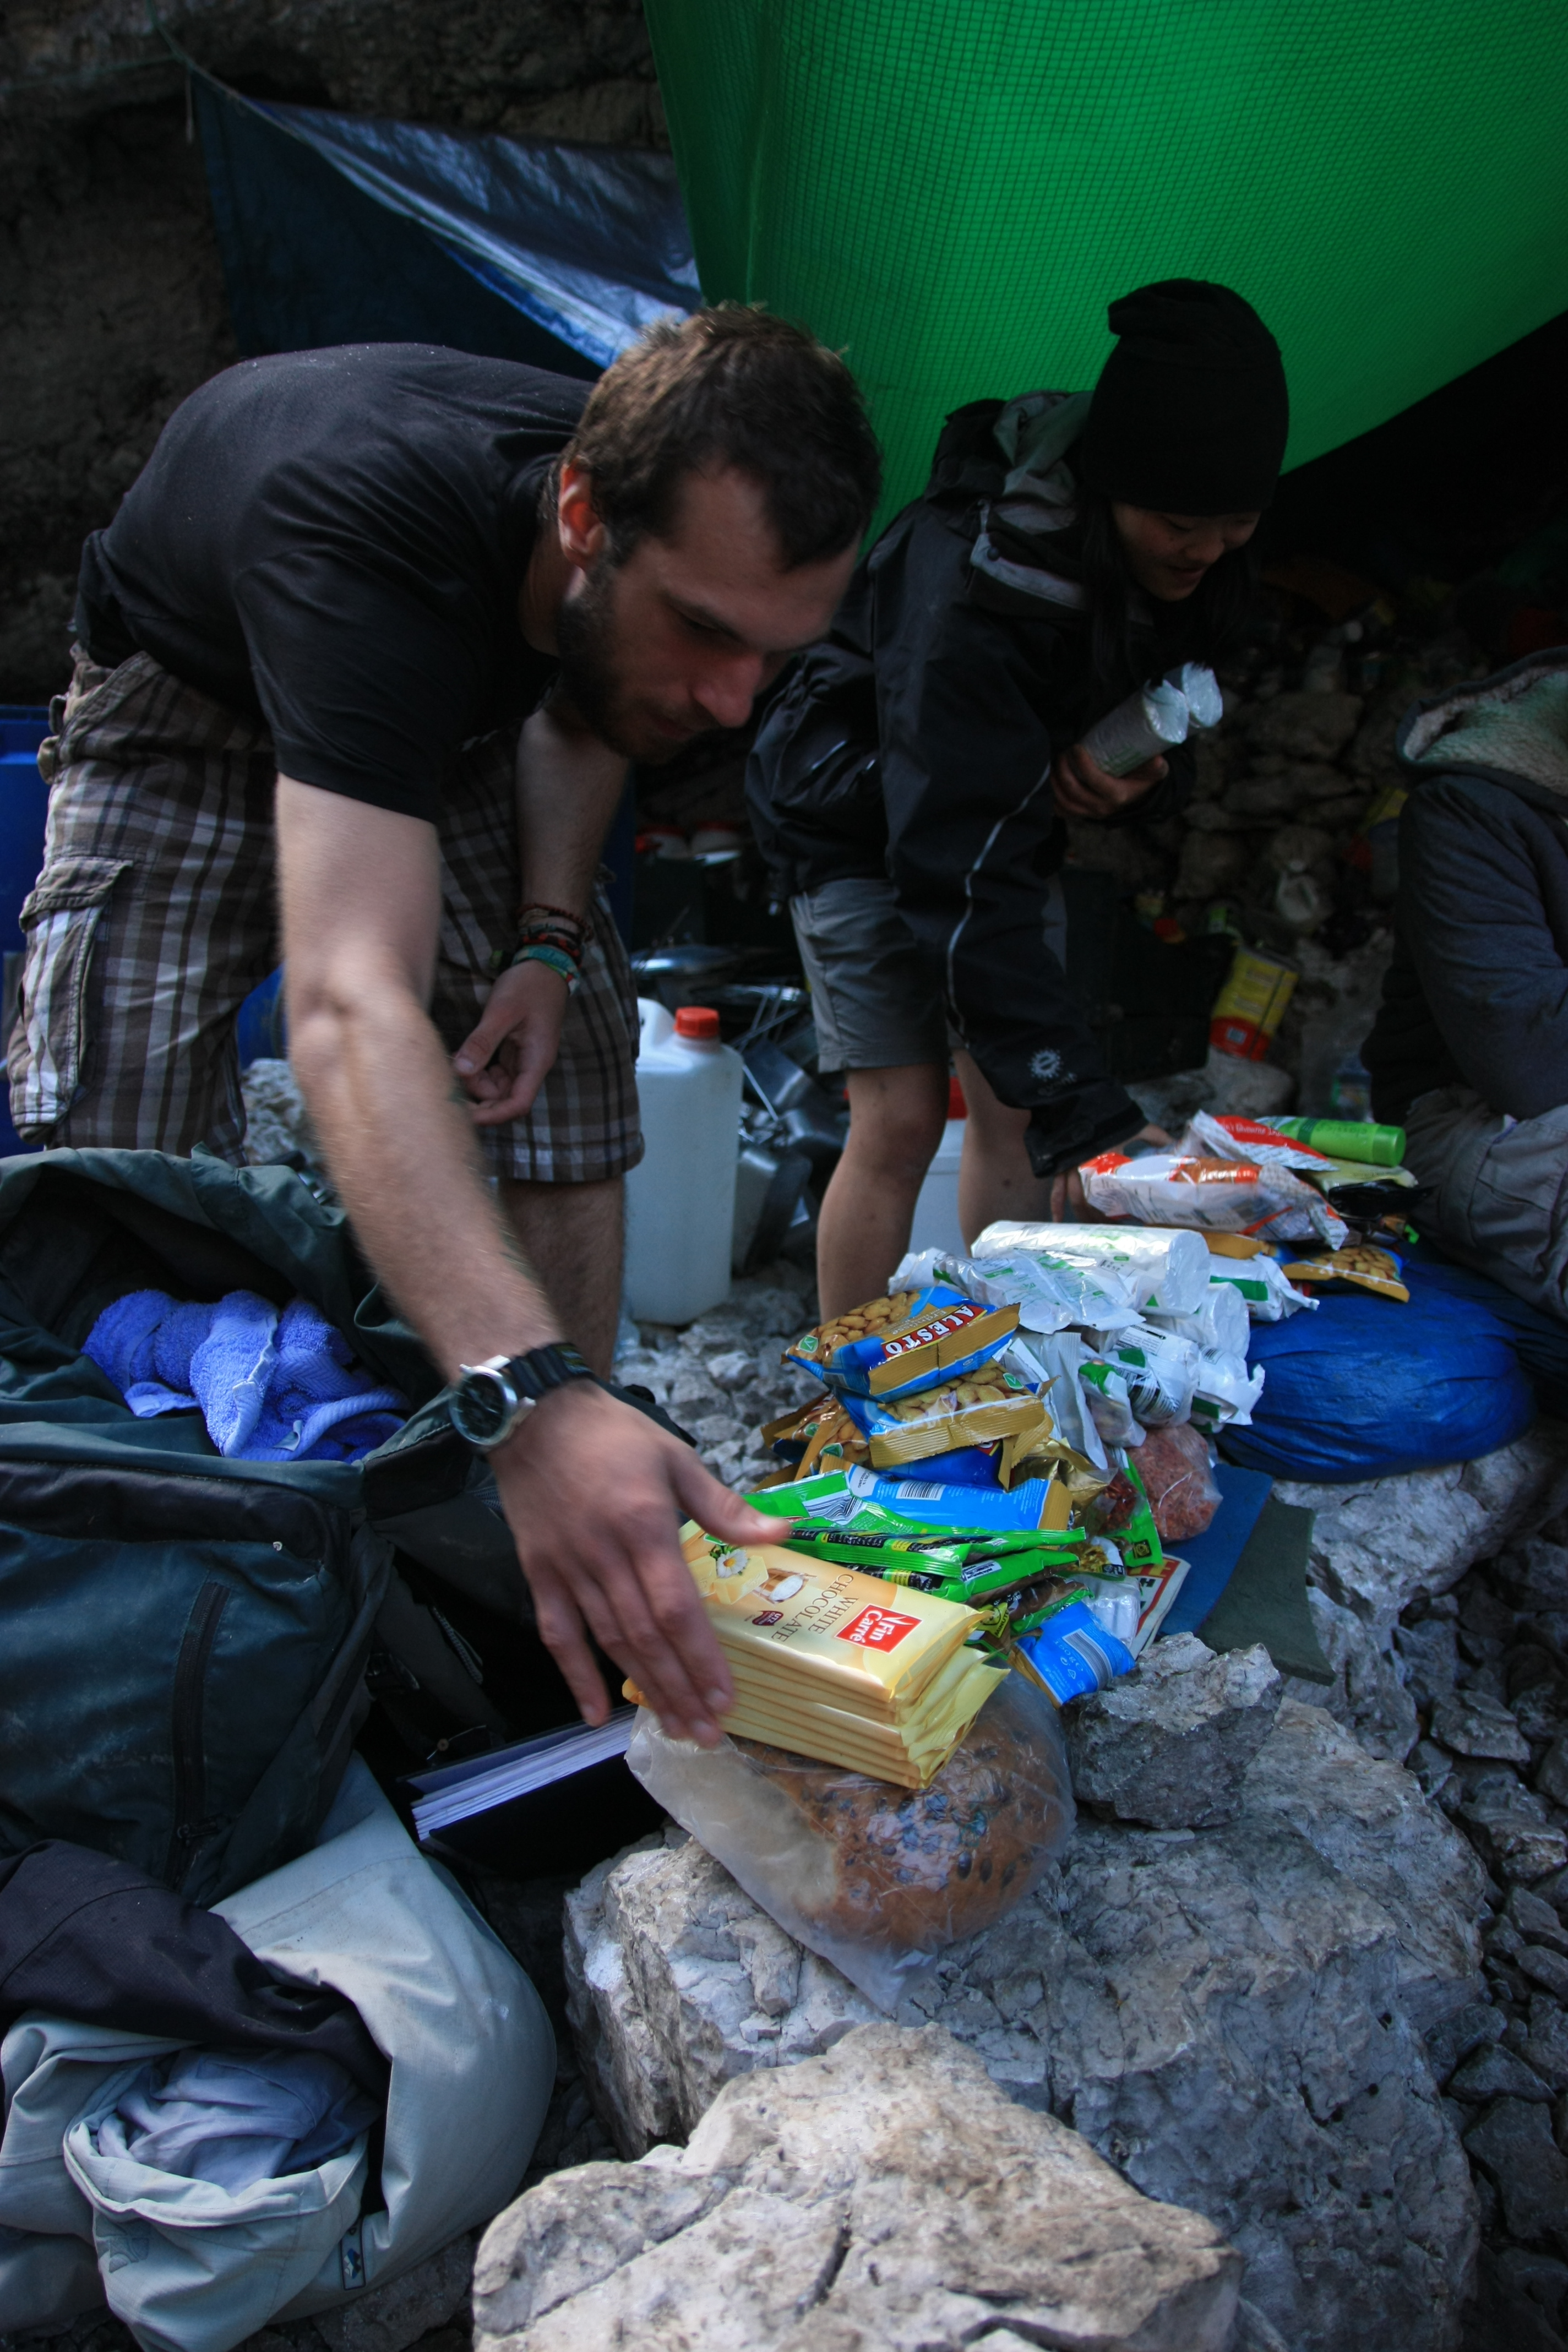
\includegraphics[width=\linewidth]{2012/piss_bandits/2012-07-29-1015-GergelyAmbrus-IMG_2065--orig.jpg}} 
 \caption{Niko and Clare unload the contents of their rucksacks after a carry (including fresh bread!), stocking up supplies in the bivi. \pic{Gergely Ambrus}}
 \label{carry unload}
\end{marginfigure}

The prospect of spending a second summer camped on \passage[mountain]{Migovec} carried with it an entirely different mix of emotions than those preceding my first year. Gone were the fears of the unknown, replaced with an exciting familiarity that may be felt when meeting an old friend. Perhaps more importantly though, was a new sense of independence and confidence that had been lacking throughout my first year. No longer was there a reliance on someone to show me the ropes and, as such, I found myself fitting into the carries and rigging that typify the beginning of the expedition, feeling like an experienced member of the team. Bivi life was great.

My sleeping arrangements were shared with Nico, an arrangement that
benefited the rest of the expedition, as our messiness and stench was
confined to a smaller area of the mountain. Our general hygiene levels
and lack of experience lead to us christening our team as the `piss
bandits.' We seemed to get on well, his laid-back style balancing my
seriousness, and as we were both looking for that `next level of
expedition independence' we decided to form a two man team to head down
to camp and have a taste of pushing.

The focus of our first pushing trip was to be an area past the \passage{Red Baron}
chamber named \passage{Queen's Road}. We had been told of a short pitch with a
possible continuation at the bottom. Simple, immediate access to virgin
cave; perfect.

Needless to say, our lack of experience made the whole process take much
longer than we had initially thought. A dodgy bolt was placed by Nico
before we swapped rigging duties and I placed a suspect deviation that
allowed access to the bottom of the pitch. Immediate gratification was
not found as the next section, despite being a small drop, required a
bolt to be placed in an awkward, narrow position. Cussing ensued as Nico
placed the bolt and wriggled his way down. Thankfully, the space seemed
to open and a further 5 m pitch promised open walking passage at the
bottom.

\margininbox{Why the face?}{
     \begin{itemize}
    \item Jonathon Hardman
    \item Nikolas Kral
    \end{itemize}}{\explo}

Now feeling much more relaxed bolting, I hurried down the next pitch to
find a large boulder filled chamber. We shouted to each other with
excitement and continued down the chamber to find a disappointing
boulder choke that barred the way on. Being the `piss bandits,' we
marked our territory before deciding it was time to head out, surveying
along the way. On our way out, we checked another continuation further
along the \passage{Queen's Road} passage (up \passage{Hot Pants}) that seemed very promising
if bolt climbed and made a note to tell the others.

\tweet{7:17PM Jul 29, 2012}{HOT PANTS pitch dropped into WHY THE FACE? (WTF) unstable collapse. Bolt climb made in the chamber above the traverse.}

The next few days camping were awful as the wind picked up on \passage[mountain]{Migovec}
and I found myself unable to sleep without being hit repeatedly by the
side of our collapsing tent. Needless to say, we headed back down having
had little sleep, eager to escape the miserable weather. During our
absence underground, Oli and Thara had attempted to complete the bolt
climb and had unfortunately run out of time before completing it.



\begin{figure*}[t!]
\checkoddpage \ifoddpage \forcerectofloat \else \forceversofloat \fi
   \centering
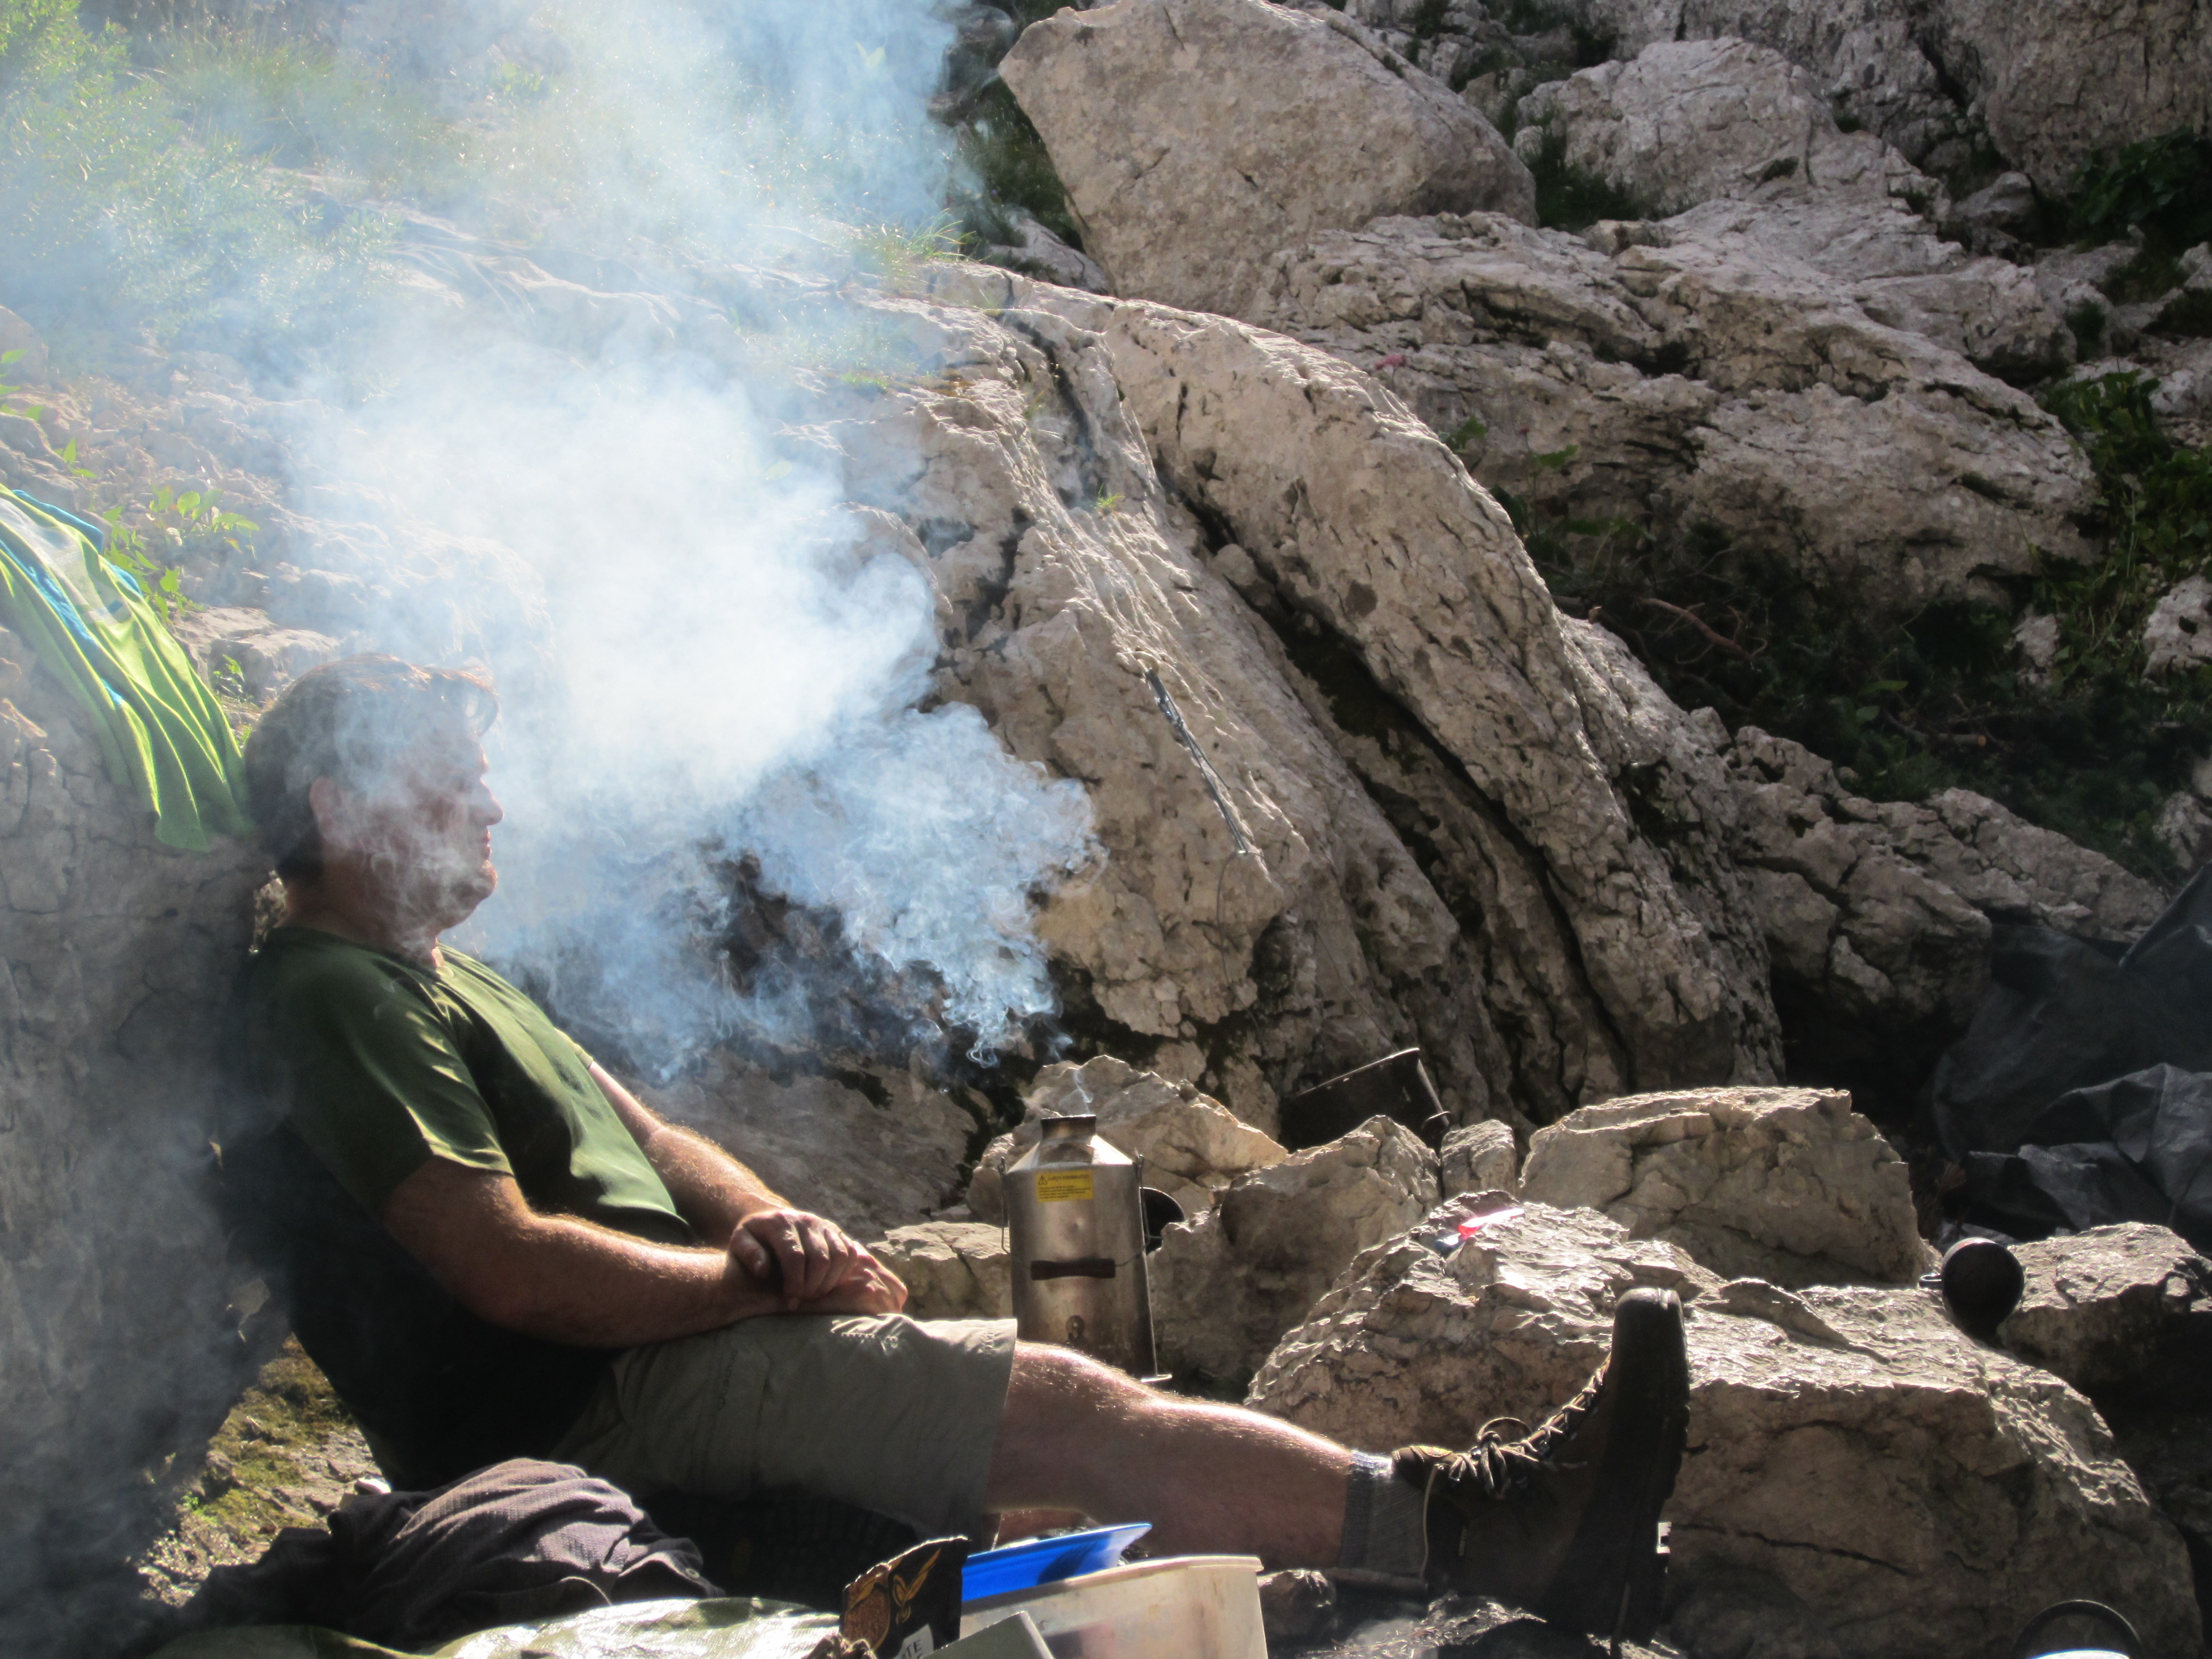
\includegraphics[width = \textwidth]{2012/piss_bandits/2012-07-28-1835-TharatornSupasiti-IMG_0111--orig.jpg}
\caption{Alongside all the obvious dangers, at times the wind also makes certain seats in the \passage{Bivi} more hazardous; here, Dewi Lloyd (in the tea seat) is harassed by smoke from the Kelly Kettle. \pic{Tharatorn Supasiti}} \label{kettle smoke}
\end{figure*}

Myself and Nico hurried up \passage{Hot Pants} to the climb and I set up off the
rope. Placing a couple of bolts to traverse left to a ledge I was faced
with a steep step followed by a muddy slope to the top of the pitch.
Having tried to a place a bolt in the friable, muddy rock I gave up and
clambered up the step and the slope, feeling confident that the climbing
skills I had acquired in \passage[town]{London} bouldering gyms were enough to ensure
safety. In hindsight they probably weren't as I awkwardly fell up the
slope like a new born calf just on the edge of physical control.
Standing at the top, adrenalised, the passage opened out into a large
walking passage similar. There were two extensions, one upslope and one
downslope and both seemed extremely promising. As I placed a bolt,
myself and Nico yelped to each other, discussing what we may find. This
was it, this was our first taste of promising lead!

\margininbox{Peep Show}{
     \begin{itemize}
    \item Jonathon Hardman
    \item Nikolas Kral
    \end{itemize}}{\explo}

First we headed downslope into a large boulder filled chamber that Oli
and Thara had asked us to christen `\passage{Peep Show}.' It was as the
piss bandits had hoped, easy pushing for a few hundred metres before the
passage ended in a boulder choke, just like our previous `lead'.
Nevertheless, the boulders here were much larger and the chamber floor
was built like a rabbit warren. The wind drafted in a small hole at the
limit of the chamber that Nico attempted to squeeze into. The
continuation narrowed within a few metres to the point where Nico could
not continue and, with a lot of writhing and whimpering, he navigated
his way back out. Being of the larger build, I didn't stand a chance.
Needless to say, we were gutted, however, this time we had a plan B.


    \begin{figure*}[t!]
\checkoddpage \ifoddpage \forcerectofloat \else \forceversofloat \fi
\centering
\begin{subfigure}[t]{0.328\textwidth}
\centering
\frame{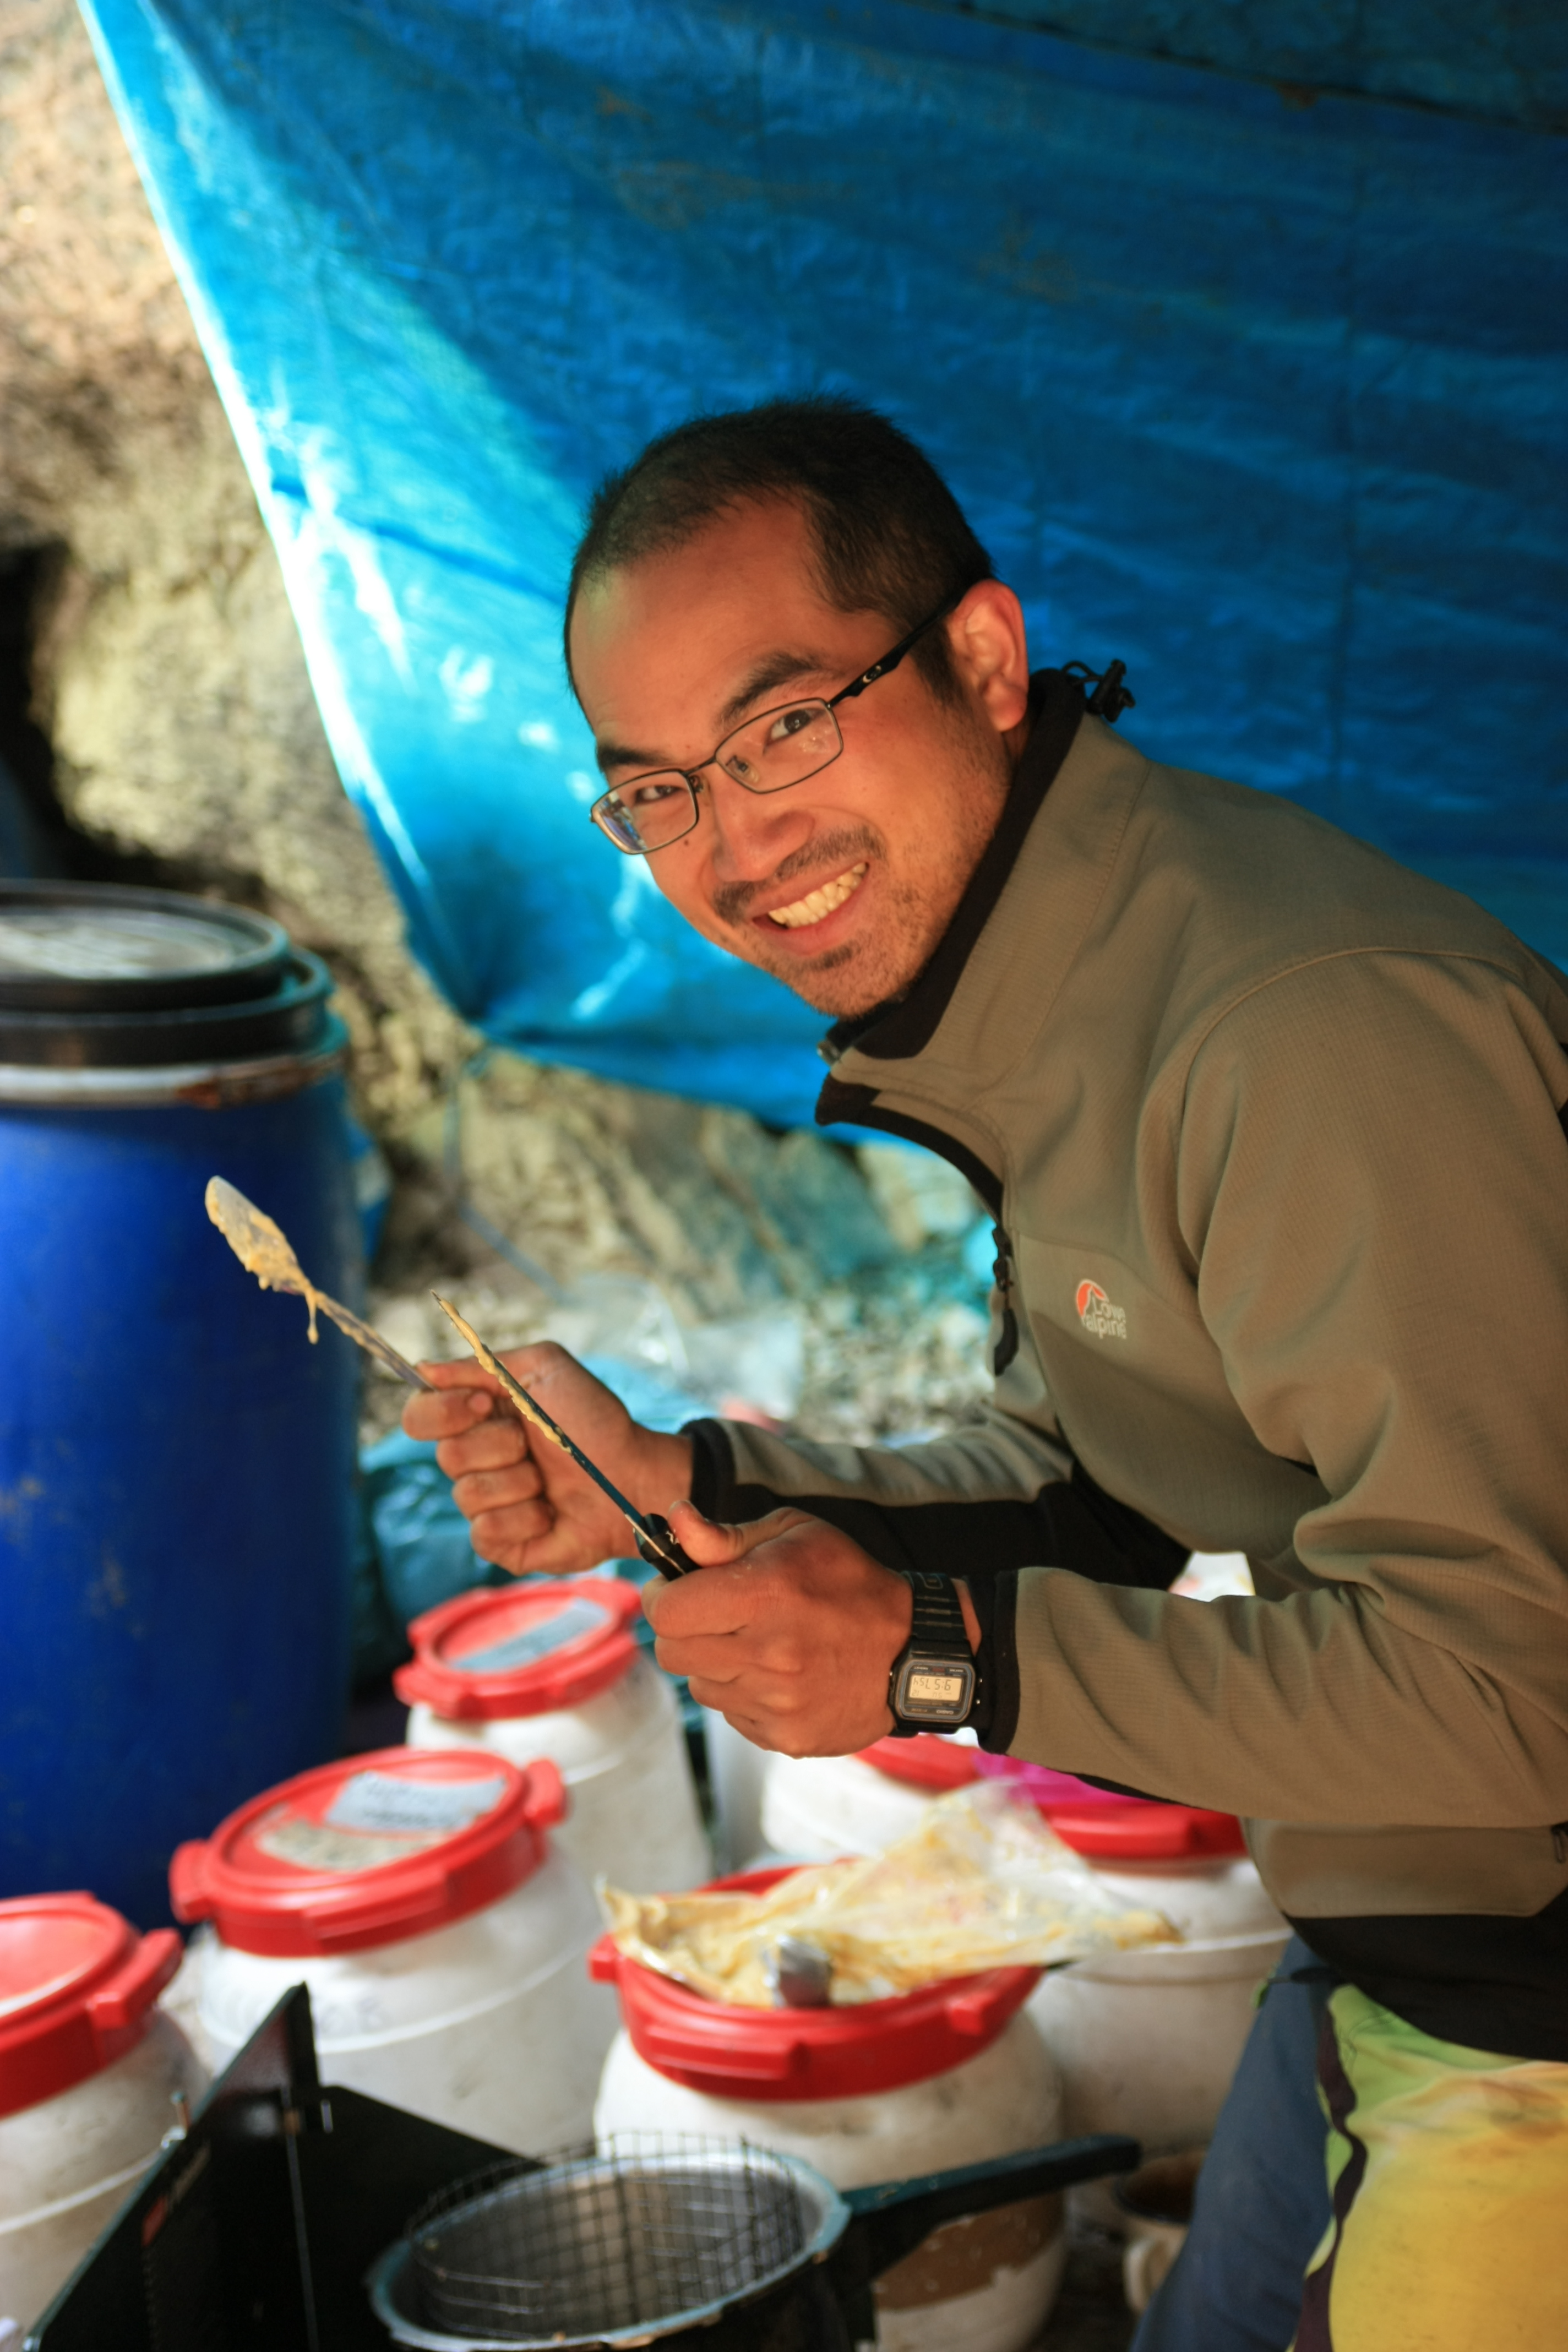
\includegraphics[width=\linewidth]{2012/piss_bandits/2012-08-12-0100-GergelyAmbrus-IMG_2453--orig.jpg}}
 \caption{}\label{thara bivi}
\end{subfigure}
    \hfill
    \begin{subfigure}[t]{0.662\textwidth}
        \centering
        \frame{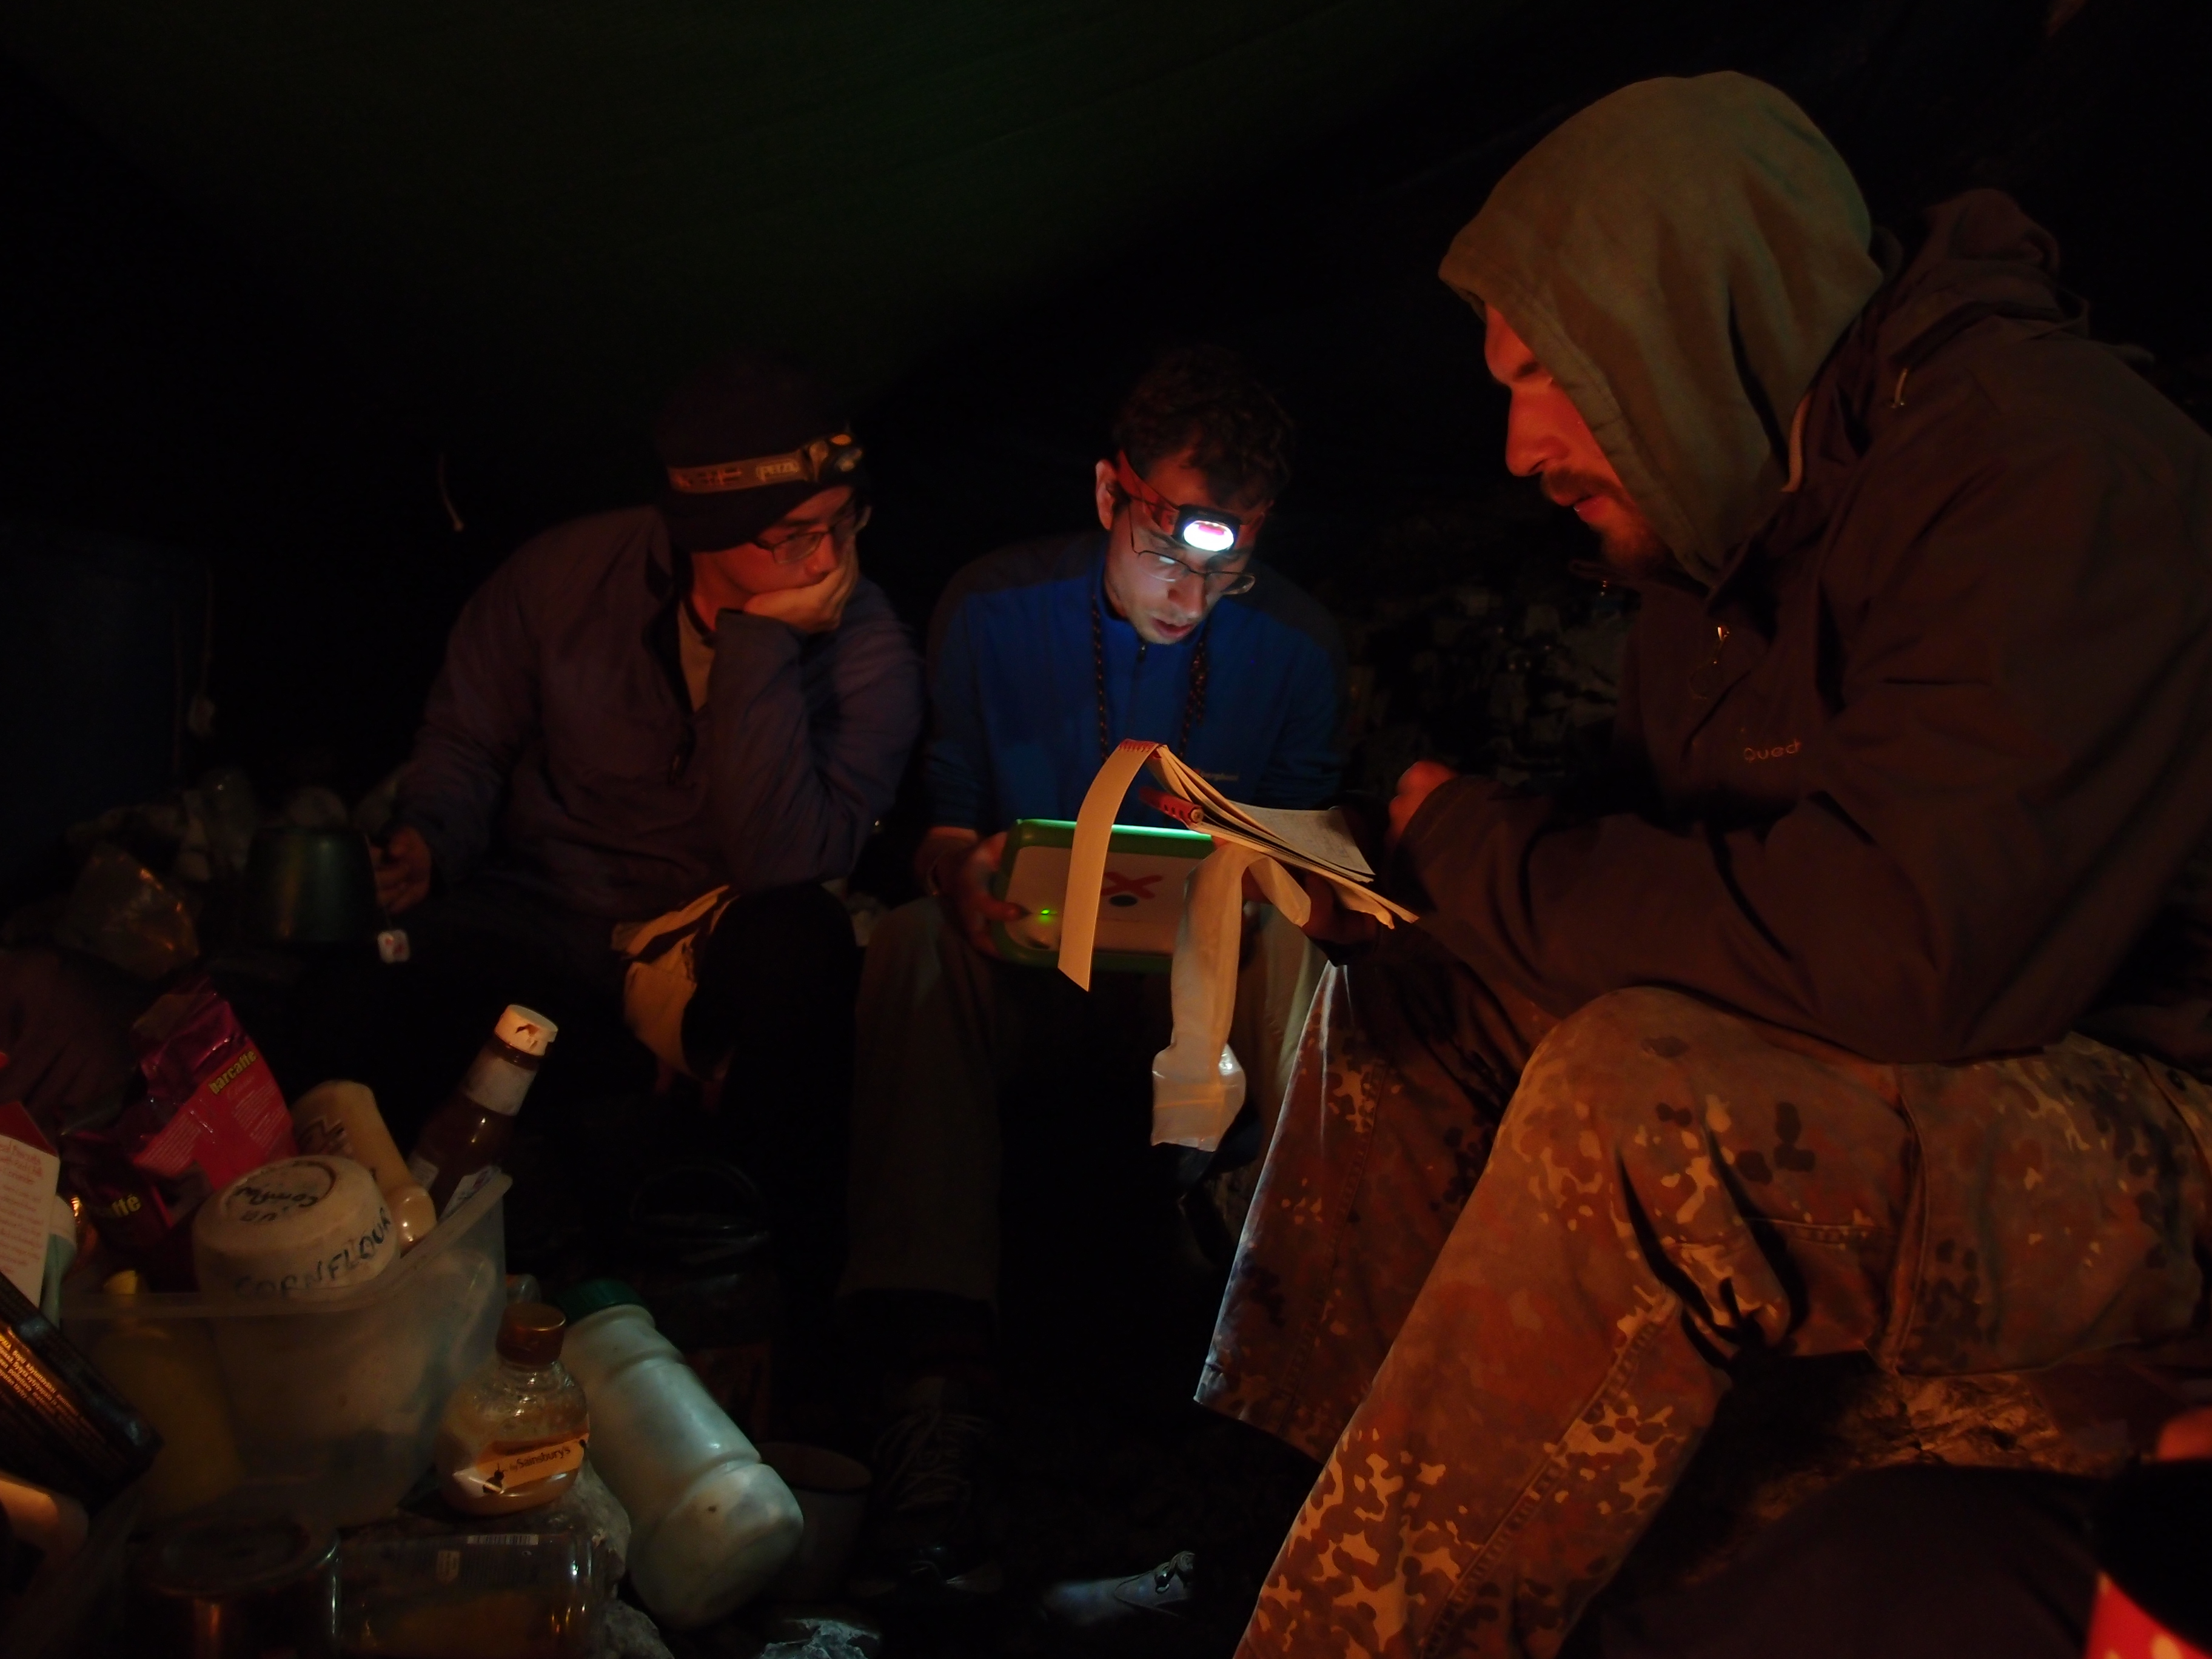
\includegraphics[width=\linewidth]{2012/piss_bandits/2012-08-03-2207-AndyJurd-P8033218--orig.jpg}} 
        \caption{} \label{clewin niko data}
    \end{subfigure}
    
    \vspace{0.3cm}
    \begin{subfigure}[t]{\textwidth}
    \centering
        \frame{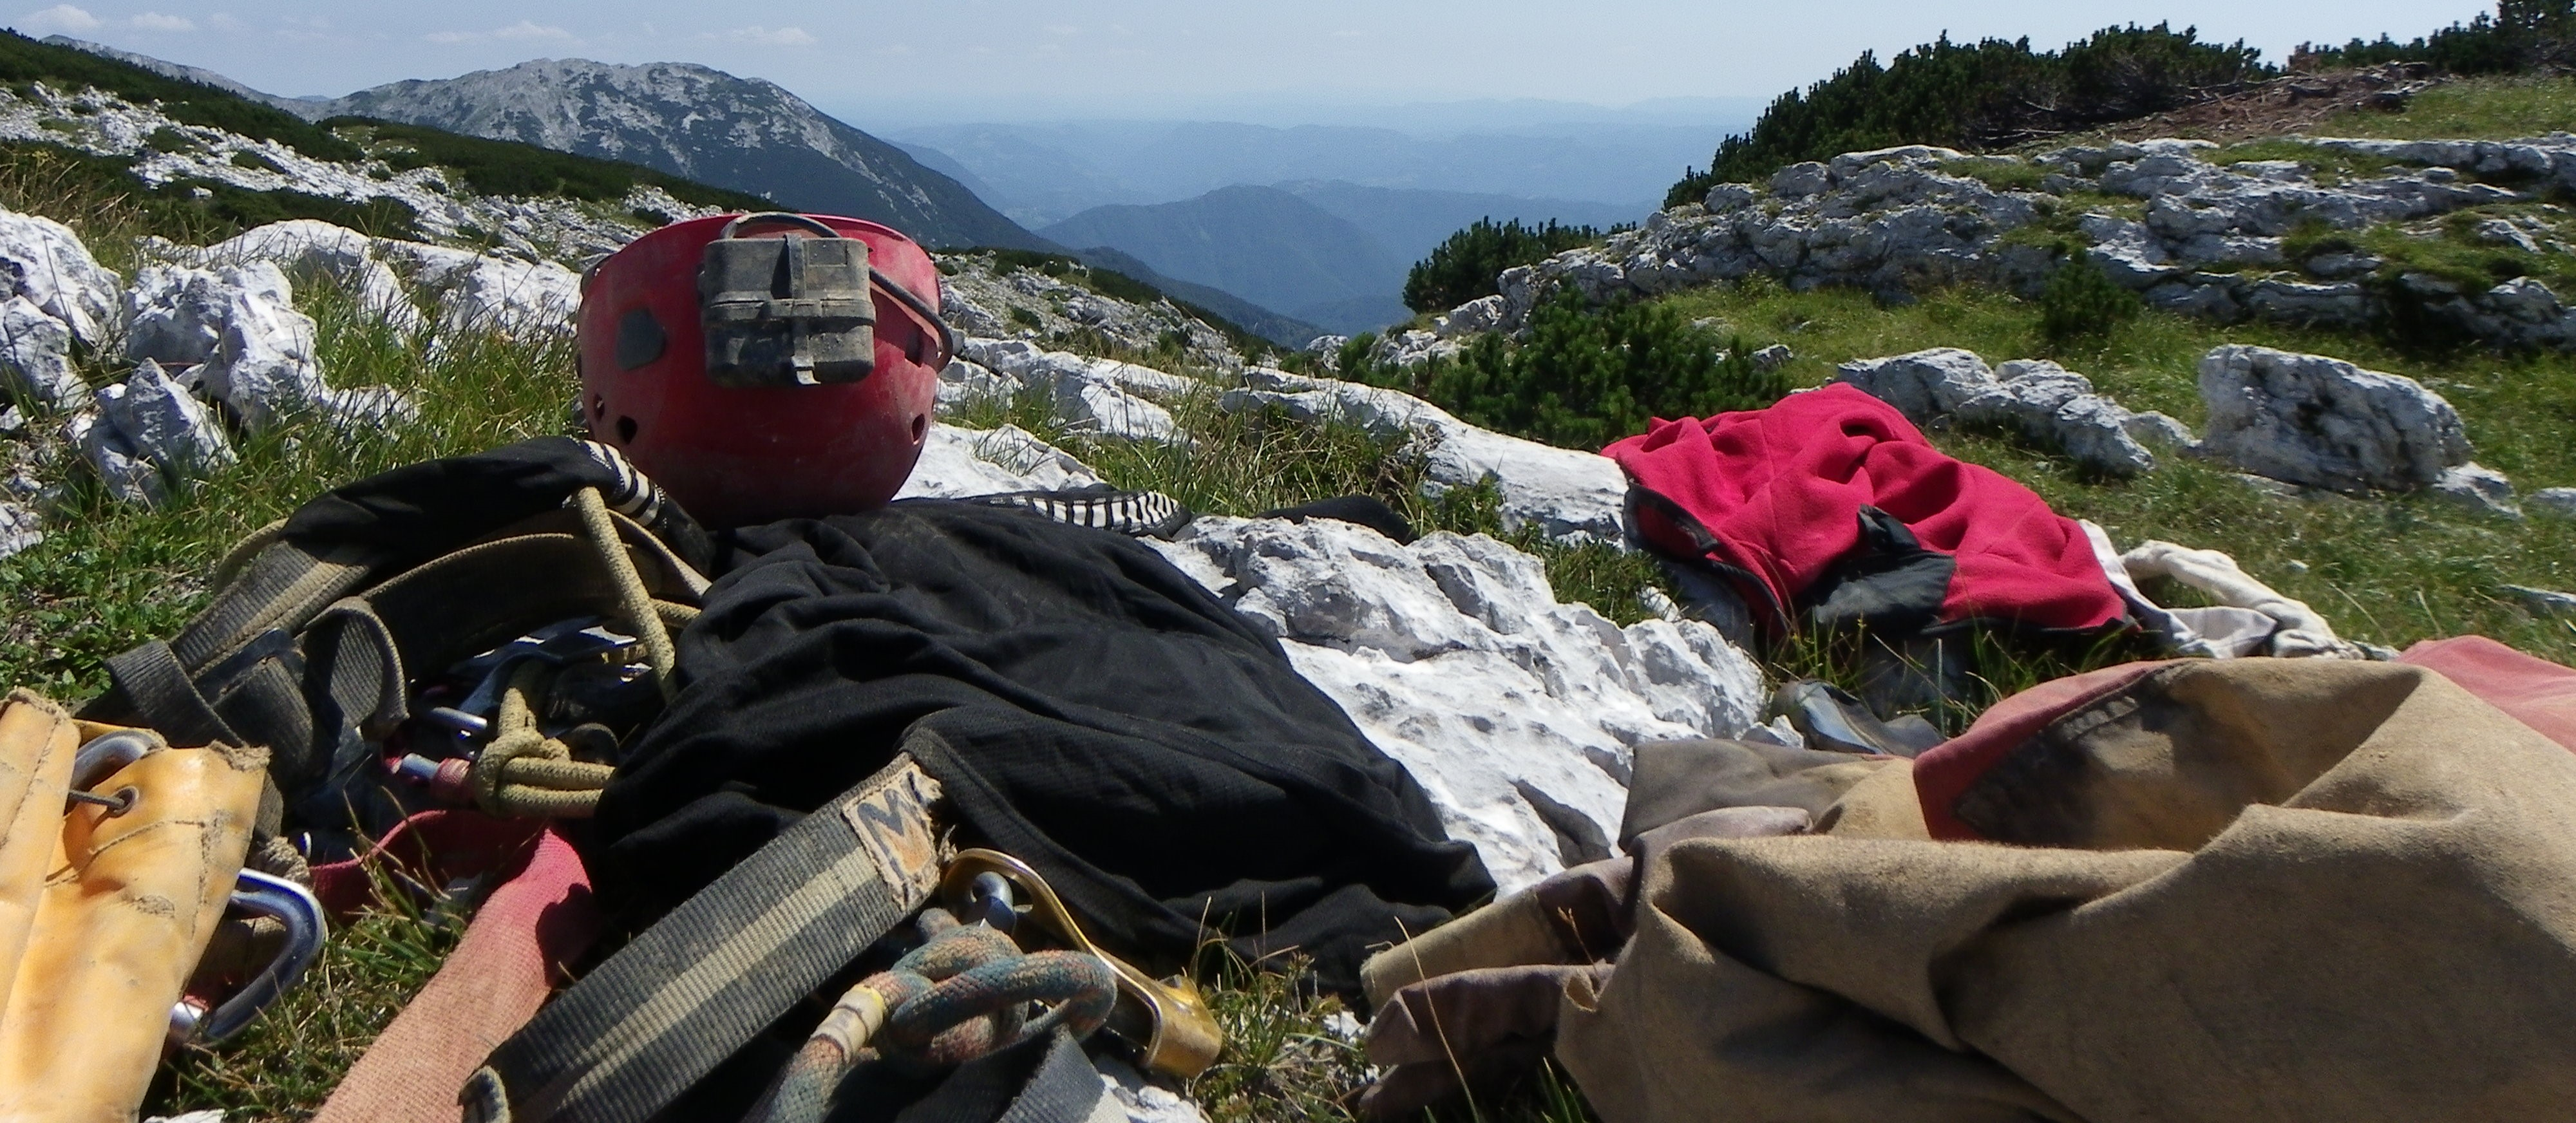
\includegraphics[width=\linewidth]{2012/piss_bandits/2012-08-08-14.53.18-Rhys Tyers-Pentax X90-IMGP3338--orig.jpg}} 
        \caption{} \label{drying gear}
    \end{subfigure}
    \caption{
    \textit{(a)} Thara cooking in the kitchen of the \protect\passage{Bivi}. \pic{Gergely Ambrus}
    \textit{(b)} Thara looks on as Clewin and Niko enter survey data into the laptop around the stone table. \pic{Andrew Jurd}
    \textit{(c)} Gear must be dried in any snatches of good weather in between caving trips. \pic{Rhys Tyers}}
\end{figure*}


The upslope continuation, that was later named \passage{Undercover Squirrel}, was
much more fun. The passage was similar to that of \passage{Hot Pants} and, whilst
mostly walking passage, there were a few muddy slopes and a couple of
climbs that made the passage much more sporting. One, in particular,
required us to wedge our body against the wall and slide down a muddy
slope, just in control until a rocky step was reached that could then be
clambered down. On the way back, such climbs proved more worrying. We
continued upwards until we reached a chimney that could be climbed up
into a large mud bedding plane with another climb up to a small window.
Unfortunately, another bolt climb was required and we surveyed our way
back out, pleased with our efforts. Whilst there was the absence of a
large, billowing draft, the lead nonetheless continued into blank
mountain.


\margininbox{Undercover Squirrel}{
     \begin{itemize}
    \item Jonathon Hardman
    \item Nikolas Kral
    \end{itemize}}{\explo}

Back at underground camp, a rather cold and miserable Tetley and Rhys
arrived bringing tales of poor weather up top. Whereas during my first
year underground camp had been a cold, remote area that had been
psychologically troubling to spend a great deal of time in, it had since
transformed into a place of considerable comfort and warmth; a second
home. As such, it was with displeasure that we pried ourselves away from
the soupy, cheesy, fishy, noodley smash and headed out from camp
\passage{X-Ray} to the surface.





Emerging at the top of \passage[mountain]{Migovec}, we found the mountain deserted. As the
weather had worsened, the rest of the expedition had fled the mountain
for a mid-Expo break. The site wasn't exactly welcoming and, with the
sun beginning to set, we made the decision to jog down to \passage[town]{Tolmin}. We
hurried down in the night, lighting the paths with our head torches,
fuelled on by prospect of a cold beer in warm, civilised abodes. We
passed the other cavers as they sat at a restaurant near the \passage{Devil's
Bridge} (Nico, ``Heeeyyy maaannn, is that the ootthhheers?''), yet,
thinking that we were hallucinating we rushed past, down to \passage[town]{Tolmin}. As
such, we arrived at \passage{Tetley's} house, locked out. We collapsed in two
content heaps and waited for others, considering the improbability that
6 hours previously, we had been 600 metres underground.

\name{Jonathon Hardman}


\begin{figure}
\checkoddpage \ifoddpage \forcerectofloat \else \forceversofloat \fi
   \centering
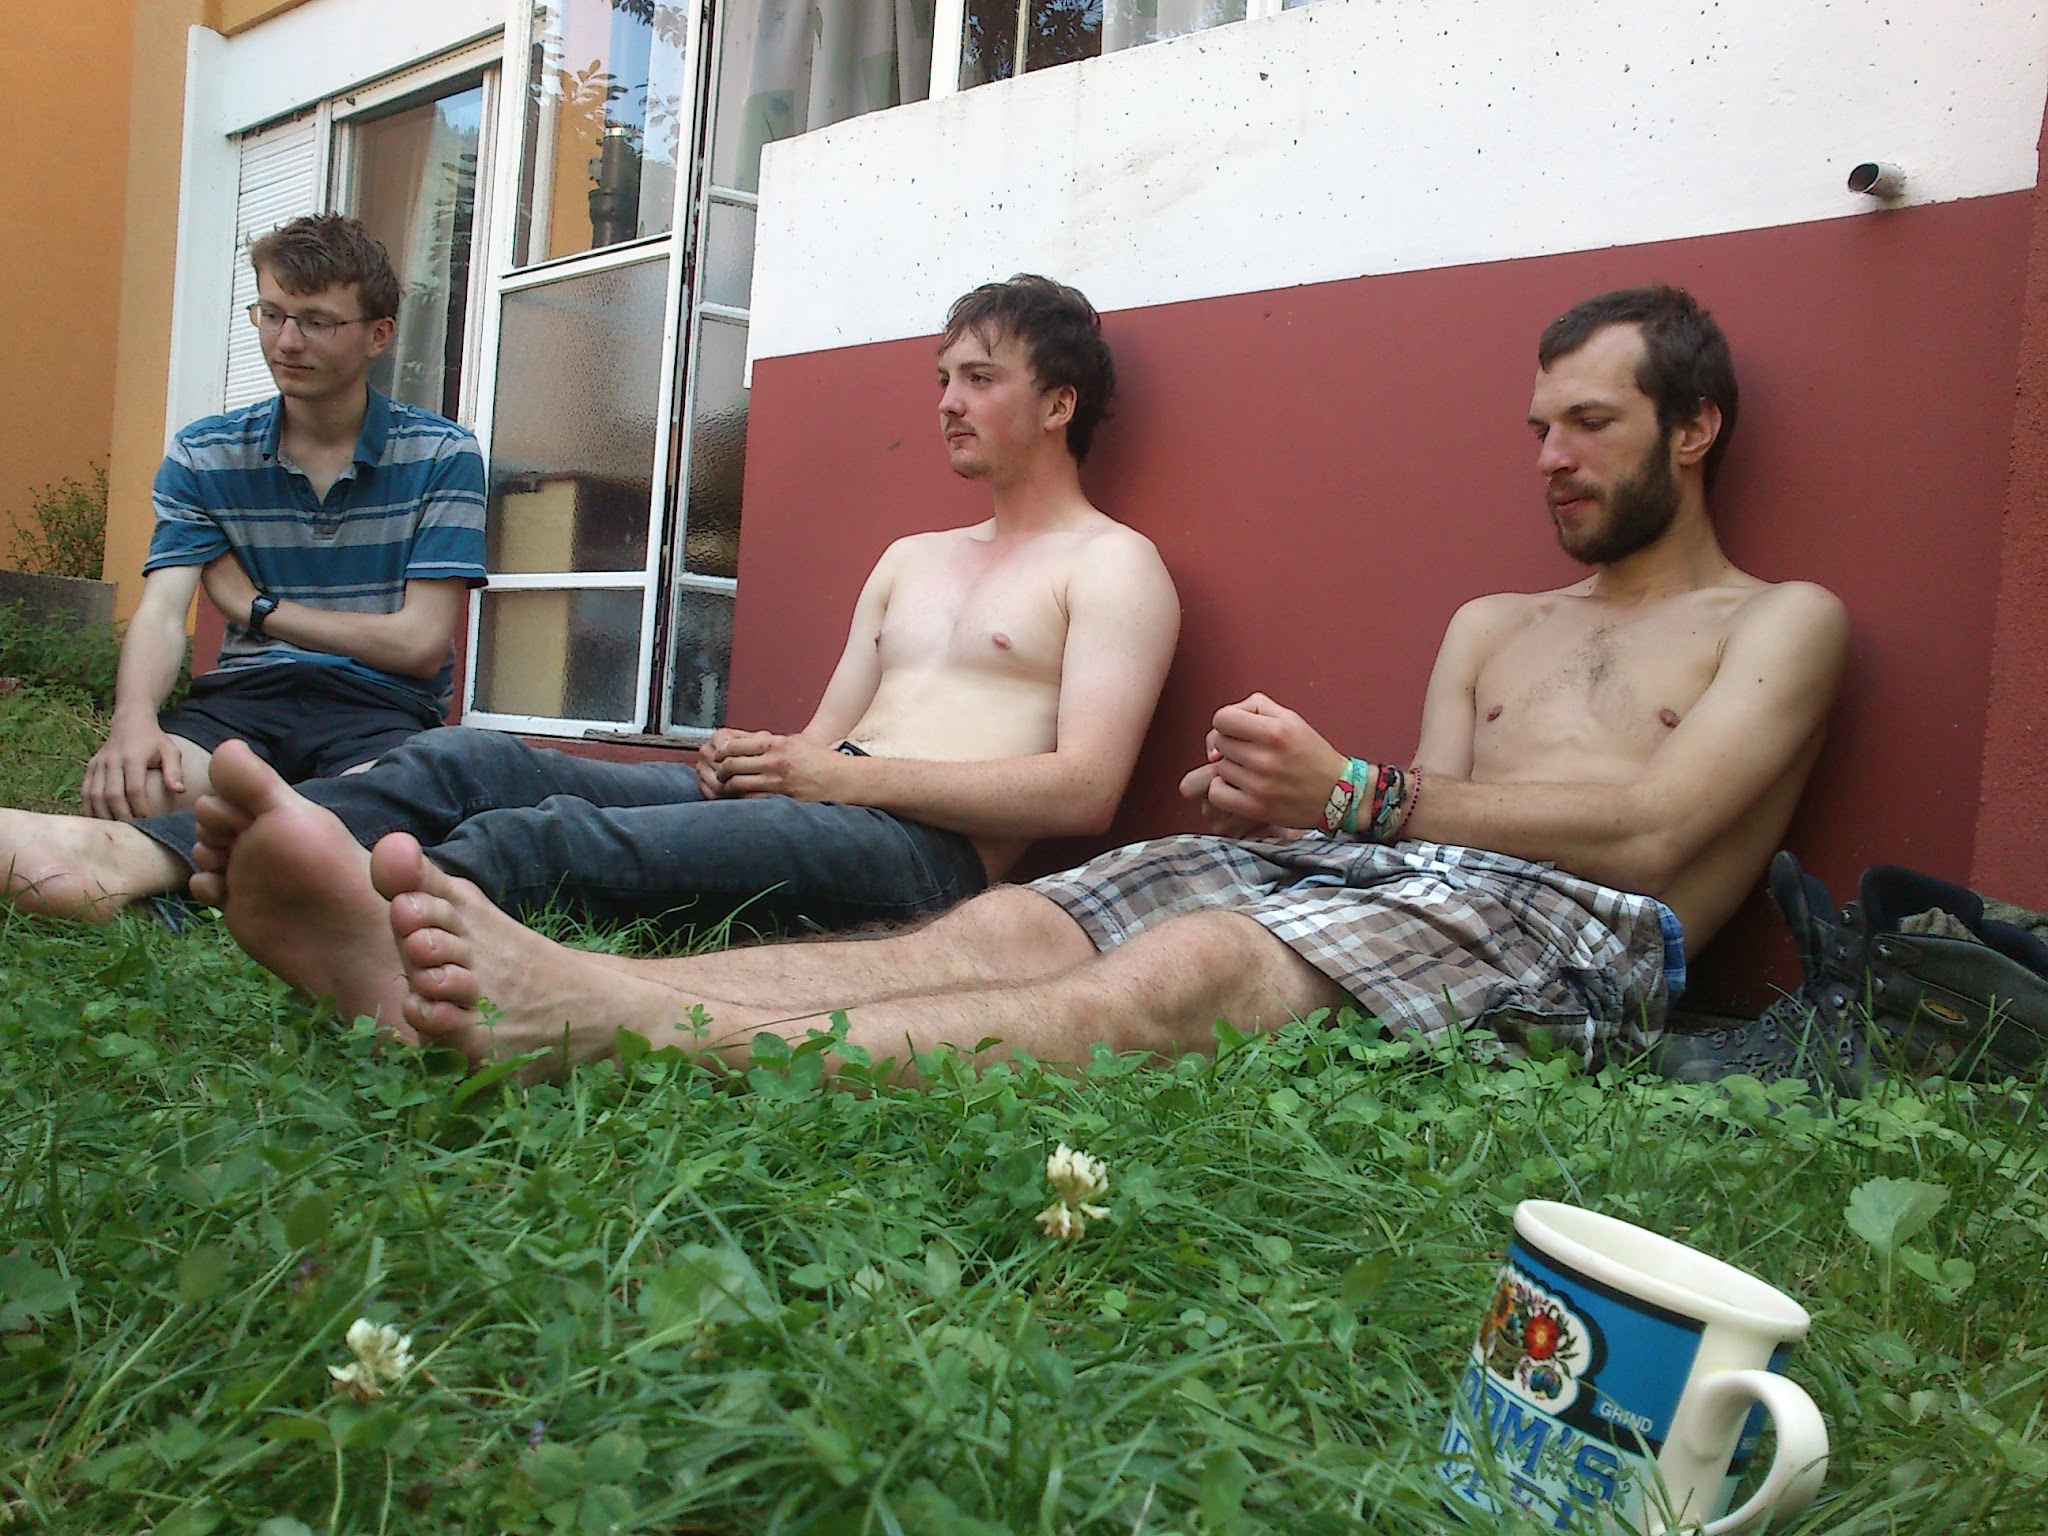
\includegraphics[width = \textwidth]{2012/piss_bandits/JarvistMooreFrost-DSC_0288--orig.jpg}
\caption{Sam Page, Jonathon Hardman and Nikolas Kral relaxing in the garden at \passage{Tetley's flat}, in \passage[town]{Tolmin}. \pic{Jarvist Frost}} \label{flat garden}
\end{figure}

\subsection{Where have all the flowers gone?}

\begin{verse}
\begin{centering}
\vspace{3pt}    

\note Where have all the flowers gone?
\newline Long time passing
\newline Where have all the flowers gone?
\newline Long time ago
\newline Where have all the flowers gone?
\newline Young girls have picked them, every one
\newline Oh, when will they ever learn? x2
\par Where have all the young girls gone?
\newline Long time passing
\newline Where have all the young girls gone?
\newline Long time ago
\newline Where have all the young girls gone?
\newline Gone for husbands, every one
\newline Oh, when will they ever learn? x2
\par Where have all the husbands gone?
\newline Long time passing
\newline Where have all the husbands gone?
\newline Long time ago
\newline Where have all the husbands gone?
\newline Gone for soldiers, every one
\newline Oh, when will they ever learn? x2
\par Where have all the soldiers gone?
\newline Long time passing
\newline Where have all the soldiers gone?
\newline Long time ago
\newline Where have all the soldiers gone?
\newline Gone to graveyards, every one
\newline Oh, when will they ever learn? x2
\par Where have all the graveyards gone?
\newline Long time passing
\newline Where have all the graveyards gone?
\newline Long time ago
\newline Where have all the graveyards gone?
\newline Gone to flowers, every one
\newline Oh, when will they ever learn? x2
\newline \textit{repeat first verse}


\end{centering}
\end{verse}

